\chapter{Improving RosettaLigand Speed and Sampling Efficiency through the Development of a Novel Sampling Algorithm}
\label{chap:lowres_paper}
\section{Abstract}

RosettaLigand has been successfully used to predict protein-ligand binding poses in a number of cases \citep{Turlington:2013et,Davis:2009fx,Combs:2013bl}.
However, the RosettaLigand docking protocol is relatively inefficient at sampling the ligand binding site space, making it unfeasibly slow for use as a \ac{vHTS} tool.
We show here that the development of a new sampling algorithm for initially placing the ligand in the protein binding site dramatically improves both the overall success rate of small molecule docking as well as speed of RosettaLigand.
The new algorithm improves the docking success rate by 10-15\% in a 43 protein benchmarking set, reduces the average time to generate a model from 50 seconds to 10 seconds, and reduces the necessary number of models to generate from 1000 to 150.
We also demonstrate that accurate initial placement of the ligand prior to full atom refinement is critical to successful prediction of an accurate binding pose.

\section{Introduction}

\subsection{Ligand docking background}

Computational ligand docking has been a historically successful method for predicting the binding pose of small molecules in a protein.
Beginning with PJ Goodford's work in computational drug design \citep{Goodford:1985bf}, many methods have been developed to predict the interactions between proteins and small molecules.
While early tools focused primarily on rigid body goodness of fit between a small molecule and a protein crystal structure, further study of the changes observed in protein conformation upon the binding of a small molecule \citep{Bystroff:1991tl} suggested that modeling of protein and ligand flexibility was important to correctly model protein-ligand interactions.

\subsubsection{An overview of popular ligand docking tools}

Over the past several decades, numerous tools have been developed to attempt to better address the ligand docking problem.
DOCK \citep{Ewing:2001wu}, FlexX \citep{Hindle:2002tk}, AutoDock \citep{Morris:1998vi}, and Glide \citep{Friesner:2004hm} are currently among the most popular tools.
They utilize a wide range of protein representations, sampling algorithms and scoring functions in order to accurately predict protein-ligand binding poses.
Approximations in scoring and sampling must be made in order to allow ligand binding predictions to be made in a reasonable time.
To accomplish this, most ligand docking tools operate in stages, so that the size of the search space is limited as the complexity of the scoring function and sampling density within the search space is increased.

\subsubsection{Summary of popularly used docking algorithms}
Docking methods differ in their means of accomplishing this step-wise increase in sampling resolution coupled with the reduction of search space.
For example, the DOCK algorithm creates a "negative space" model of the binding site created by placing spheres inside the solvent accessible area of the binding site, and uses this model to guide docking of the ligand, while an AMBER based molecular mechanics force field is used to score the resulting binding poses \citep{Moustakas:2006fe}.
FlexX, on the other hand, represents the protein by "interaction centers" consisting of surfaces surrounding common ligand interaction groups (hydrogen bond donors and acceptors, metals, aromatic rings, etc.).
Atoms in a based fragment of the ligand are then matched to the interaction centers to provide an ensemble of potential initial placements \citep{Rarey:1996hf}.
AutoDock represents the receptor using a cartesian scoring grid populated with information from an empirically derived energy function.
A \ac{LGA} in combination with simulated annealing is then used to optimize both the ligand conformation and position \citep{Morris:1998vi}.
Glide uses a grid based representation of the protein binding site. A rapid exhaustive search is first performed to find generally favorable areas for ligand placement.
A size filter is then used to exclude areas without sufficient space for ligand placement.
Finally, \ac{MCM} of the binding pose using the grid based scoring function is performed.
The scoring girds themselves are generated using a scoring function derived from ChemScore \citep{Friesner:2004hm}.

\subsection{Performance comparison}

\subsubsection{Performance of ligand docking tools is inconsistent} 
Despite the large differences between scoring and sampling algorithm implementations across the different ligand docking tools, a blind study of ligand docking performance conducted by Davis et al. \citep{Davis:2009fx} suggested that while certain methods of docking perform better than others for a given protein target, in the aggregate, the commonly used systems have a similar range of performance.
Interestingly, while some protein systems appear to be relatively easy (Chk1 kinase) or difficult (Hepatitis C RNA Polymerase) for most ligand docking tools, the results for most systems vary depending on the ligand docking tool.

\subsection{Limitations of the RosettaLigand low resolution docking step}

\subsubsection{Introduction to the RosettaLigand docking process}
As currently implemented, RosettaLigand consists of a two stage docking process consisting of an initial placement stage followed by a refinement stage.
The overall effect of the initial placement algorithm is to place the ligand in a non-clashing position at random.
To accomplish this, the initial placement algorithm consists of three steps, which were initially described in Davis et al. \citep{Davis:2009bf}
The algorithm uses a binary scoring grid to identify non-clashing regions of the protein.
The binary scoring grid consists of "attractive" rings between 2.25 and 4.75 \AA\ of every heavy atom, and "repulsive" spheres between 0 and 2.25 \AA\ of each backbone heavy atom. 
The first step of the initial placement algorithm ("Translate") consists of up to 50 random translations within 5.0 \AA\ of the starting position.
After each translation, the heavy atom closest to the geometric center of the ligand, termed the "neighbor atom" is scored using the binary scoring grid.
If the score is -1 or 0 (attractive or neutral), move is accepted, and the translation step terminates.
The aim of the Translate step is to place the ligand in a region of the binding site that is not majorly clashing.

\subsubsection{Description of the Rotate step}
The second step in the initial placement algorithm is the Rotate step.
The Rotate step consists of up to 500 random rotations with a maximum of 360\textdegree\ from the starting orientation.
The Rotate step accumulates a set of diverse non-clashing ligand orientations, and then selects one of these orientations at random for further refinement.
The size of the set of diverse orientations is either 5 or 5 times the number of rotatable bonds in the ligand, whichever is larger.
The ligand is randomly reoriented, and then accepted into the set of diverse orientations if the following conditions are met: No atoms are located in repulsive squares, 85\% of the atoms are located on attractive squares, and the \ac{RMSD} of the new orientation with respect to all previously accepted conformations is greater than $0.65*\sqrt{number\ of\ heavy\ atoms}$.
After either 500 orientations have been created, or the maximum set size has been achieved, a random orientation from the set is selected, and the Rotate step terminates.

\subsubsection{Description of the Slide Together step}
The third and final step in the initial placement algorithm is the Slide Together step.
Due to the relatively small amount of information provided by the binary scoring grid, it is possible for the ligand to be placed in a region where it does not contact any protein atoms at the end of the translate and rotate steps.
In this case the apparent interaction energy at the beginning of the refinement stage would be 0, reducing the efficiency and sometimes causing failure in the following Monte Carlo refinement stage.
To avoid this situation, the ligand must be brought in contact with the protein.
The Slide Together step moves the ligand towards the center of mass of the protein until the full atom repulsive score increases. 
Following this initial placement, a refinement stage is carried out in which small perturbations of the ligand and repacking of the protein side-chains are performed using \ac{MCM}.
Finally, all atoms in the binding site are minimized using gradient minimization, and the final structure is scored.

\subsubsection{Possible limitations of the low resolution placement in RosettaLigand}
We hypothesize that independent sampling of translation and rotation will complicate sampling of all favorable initial placements, particularly if the ligand is not globular.
For example a rod-shaped ligand would easily enter a rod-shaped pocket but only if it is brought in the correct orientation first.
A ligand with a bent shape might require reorientation while entering the binding pocket in order to avoid clashes.
Therefore, RosettaLigand will miss out on favorable initial placements for other ligands but spend substantial time performing refinement and minimization moves on ligands placed in unfavorable initial positions.
The result of this inefficiency would be an increased failure rate as some ligands are never placed in favorable starting positions, and for other ligands an effectively increased runtime, as the number of ligand poses which must be generated to reliably produce a high quality binding pose is increased.
Lemmon et al. \citep{Lemmon:2013jd} determined that as many as 1000 models may be necessary to produce at least one high quality binding pose in a challenging docking case.
Given this, improving the efficiency of protein binding site sampling by starting from more favorable initial placements has the potential to drastically reduce the computational cost of RosettaLigand, allowing for a larger number of predictions to be made given a fixed amount of computing resources.

\section{Results}

The improved initial placement algorithm has two components: A modular grid based scoring function, and a \ac{MCM} based sampling algorithm.
Both components are fully independent.
The implementation described here allows for the rapid implementation of new score terms and sampling methodologies, and the easy integration of these methods into the existing RosettaLigand pipeline.

\subsection{Score function development}
\subsubsection{Description of scoring grids and manager}

The new score function consists of a set of scoring grids which are controlled by a scoring manager.
Each scoring grid is responsible for computing a single term in the energy function.
It consists of a 3D tensor of floating point values representing cartesian space.
It also contains functions to populate that tensor, and to score a ligand positioned in that tensor.
The scoring manager is responsible for keeping every scoring grid up to date with respect to the protein pose, and for making sure that the ligand is scored in every grid.
Additionally, the scoring manager is responsible for handling the weighting of the individual scoring terms to compute the total score.
For this study, the tensor has dimensions of 15 \AA$^{3}$ width, and a 0.25 \AA\ spacing between grid points. 

\subsection{Sampling architecture}
\subsubsection{Description of grid \acs{MCM}}
An \ac{MCM} algorithm is used to compute the initial binding pose for the ligand.
Figure \ref{fig:docking_flowchart} shows a flow chart of the overall steps in the sampling process.
At each step in the sampling process the ligand is either randomly perturbed in the binding site, or the conformation of the ligand is changed.
Ligand perturbation is performed as a combination of a random translation and rotation, and the conformation of the ligand is perturbed by selecting a random conformation from a library of pre-computed conformers.
After the perturbation, the ligand is scored using the scoring grids described above, and, the Metropolis criterion is applied to either accept or reject the new pose.
500 cycles of sampling are performed, and the best scoring ligand pose is saved.
During sampling, only the scoring grids are used to provide scoring information, and the protein is therefore rigid.
By only using scoring grid information, it is possible to perform 500 cycles of sampling in roughly 1-3 seconds.

\begin{figure}
%figure 1 in orginal paper
\centering
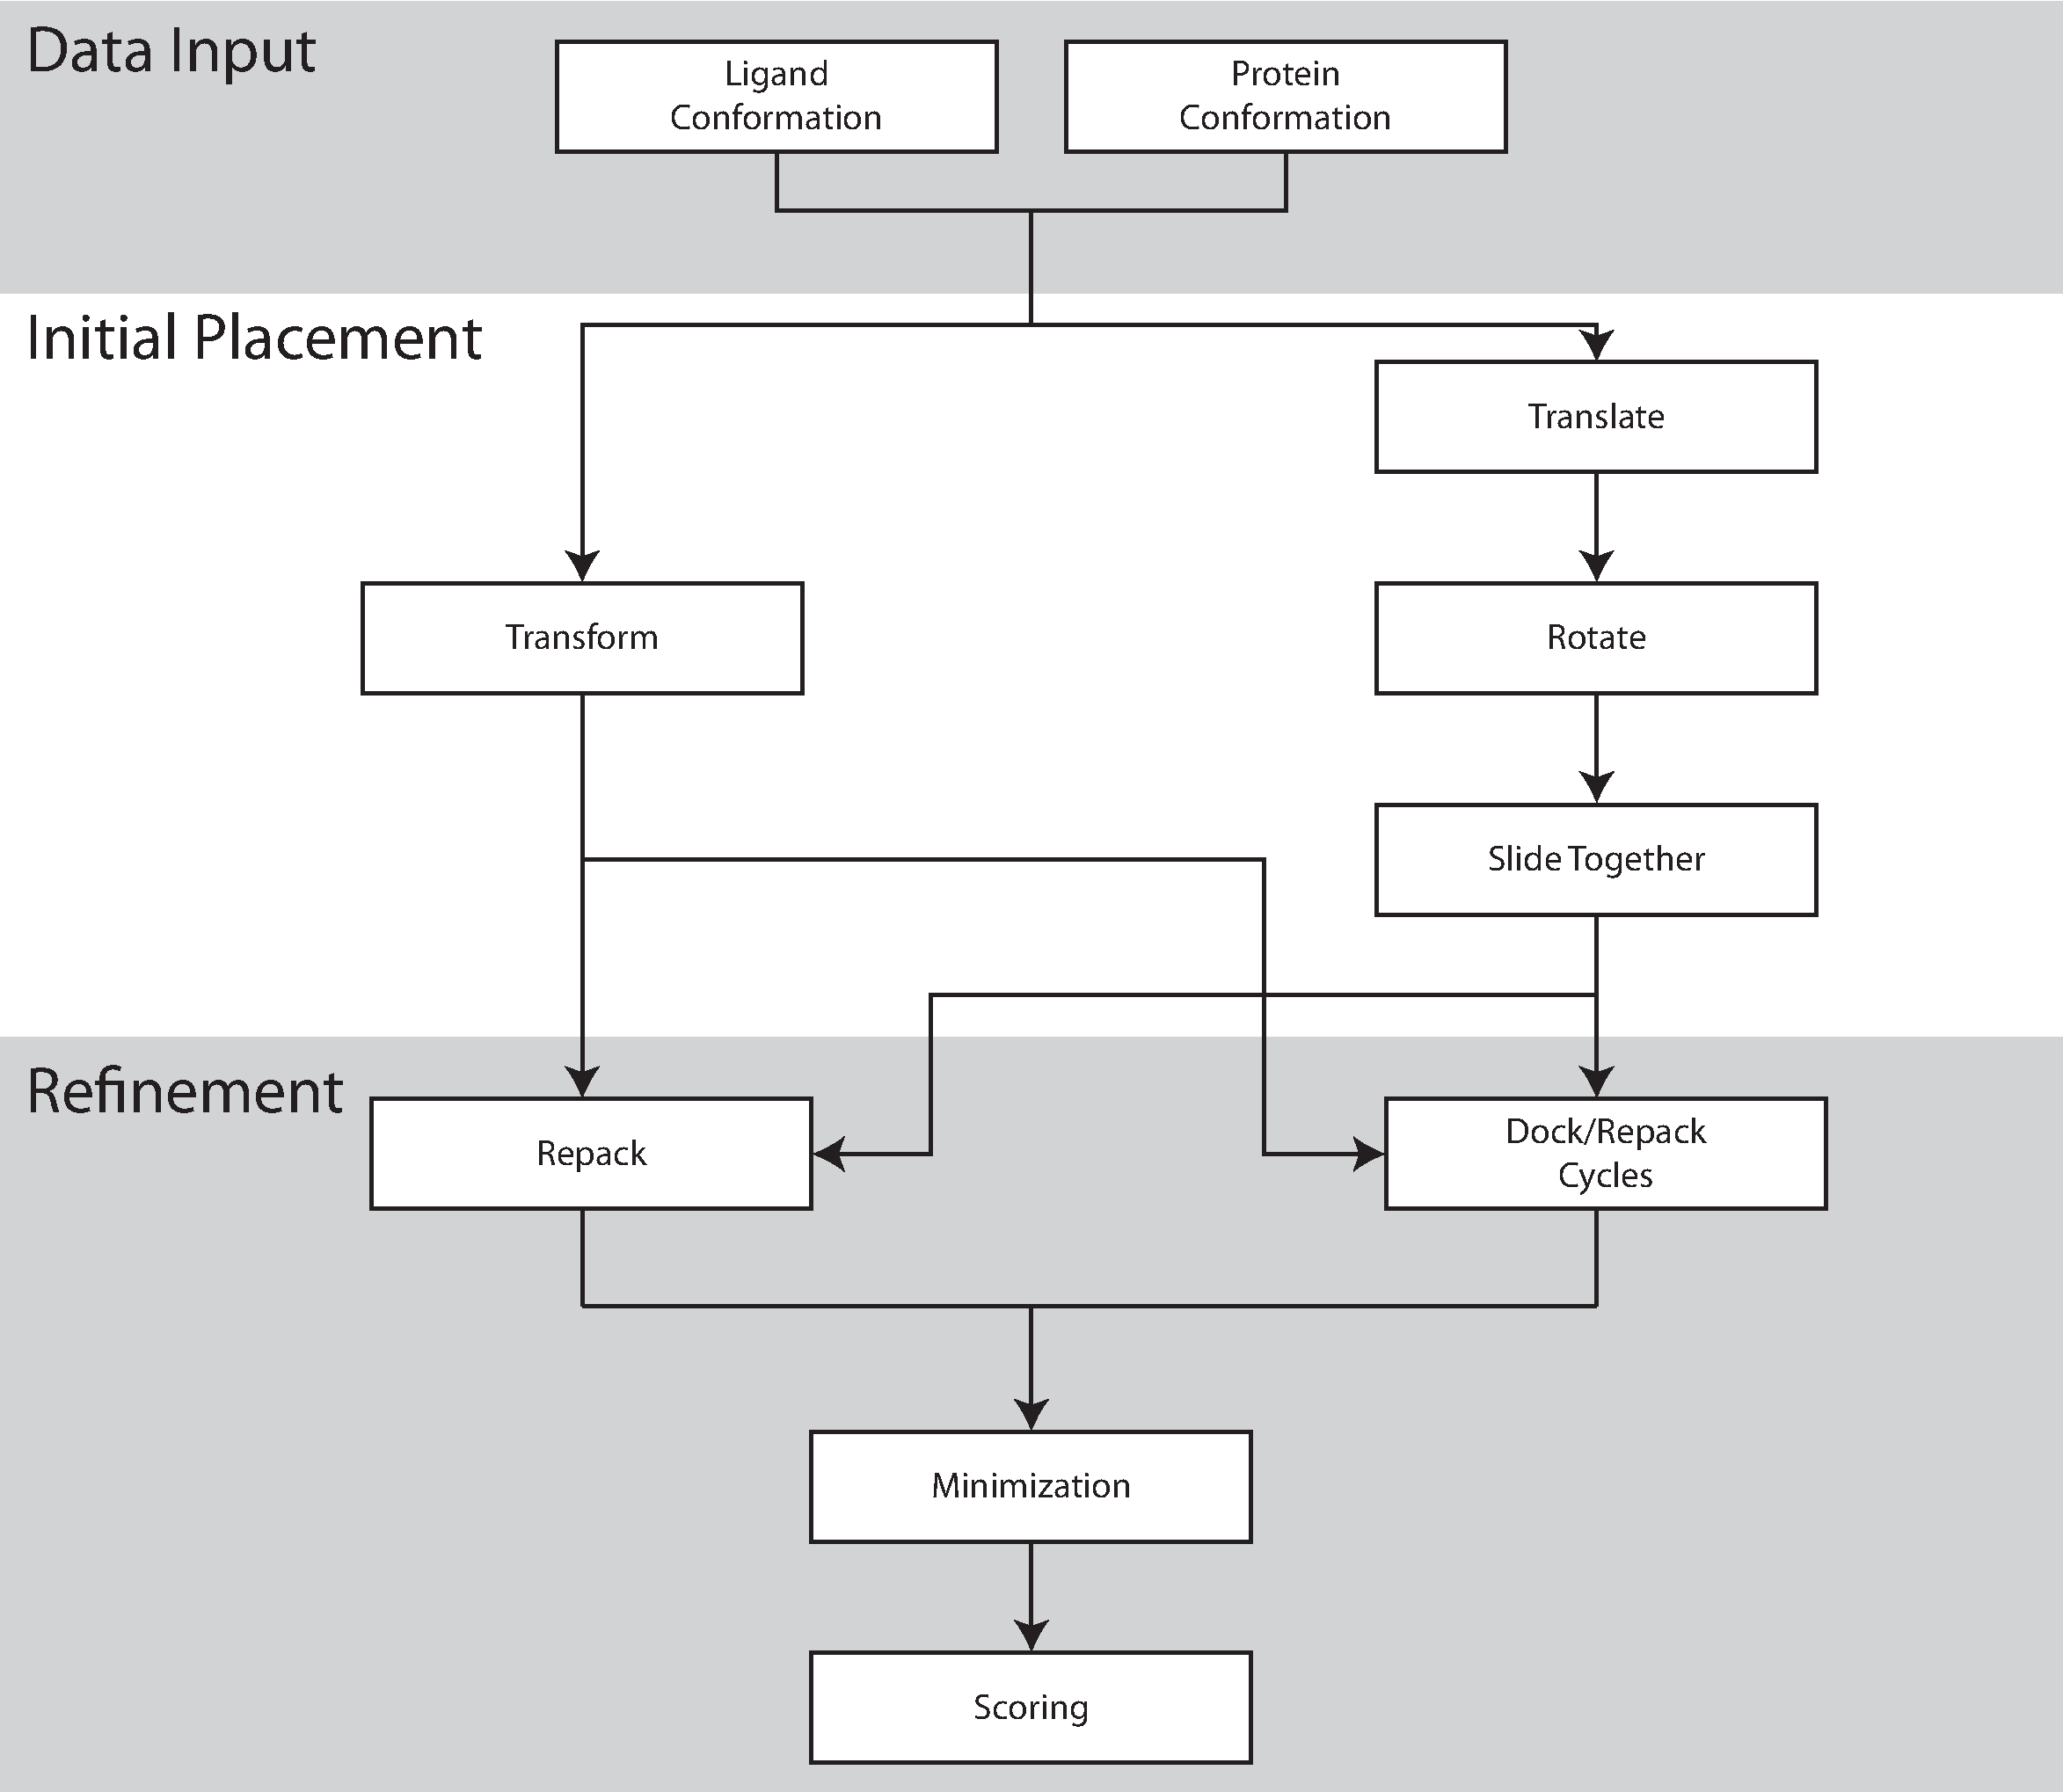
\includegraphics[width=4in]{figures/lowres/protocol_flowchart.pdf}
\caption{
A general schematic of the docking protocols described in this paper.
Because the initial placement and refinement steps are independent, the two initial placement algorithms can be combined to produce a total of four ligand docking algorithms.  
}
\label{fig:docking_flowchart}
\end{figure}

\subsection{Docking Protocol}
\subsubsection{Introduction to the docking process}
The overall docking protocol is illustrated in the schematic flowchart in Figure \ref{fig:docking_flowchart}.
The study compares different configurations of both the initial placement step and the refinement step, described below.
Complete RosettaScripts \ac{XML} files for each experiment can be found in chapter \ref{chap:lowres_capture}.
As a baseline we use the \textsc{TransRot} initial placement algorithm, where translation and rotation moves are performed separately using the binary scoring grids described by Davis et al. \citep{Davis:2009bf} and summarized in the introduction.
The specific TransRot protocol used here is originally described in Fleishman et al. \citep{Fleishman:2011ji}, and is conceptually identical to the process described in the Davis paper, though the user interface is different. 

\subsubsection{Description of the \textsc{Transform} based initial placement algorithm}

In the new \textsc{Transform} based initial placement algorithm, translation and rotation are performed simultaneously.
500 steps of \ac{MCM} are carried out.
At each step, the ligand position is either transformed, or the ligand conformation is changed using the ligand conformers described above.
When a transformation move is selected, the ligand is randomly translated within 0.1 \AA\ of its current position, and rotated within 5\textdegree.
The ligand is constrained to only move within 5 \AA\ of the starting position.
After each move, the score is evaluated as the sum of the values at each grid square occupied by a ligand atom.
The move is the accepted or rejected using the Metropolis criterion, and the best scoring accepted move after all 500 steps is returned.

\subsubsection{Description of the \acs{MCM} refinement algorithm}
During \ac{MCM} refinement, the scoring grids are not used, and the full atom Rosetta energy function is used for energy computation.
\ac{MCM} refinement consists of two steps: high resolution docking, and gradient-based minimization.
Six steps of high resolution docking are performed. The steps consist of either repacking followed by minimization, or ligand perturbation.
In the repacking and minimization step, the side-chain positions are optimized using side-chain rotamers from the Dunbrack rotamer library \citep{Shapovalov:2011bw}, and the ligand is allowed to change conformation using the pre-computed ligand conformers.
Following repacking, a gradient based minimization is applied to minimize the energy of the side-chain and ligand atoms.
In the perturbation step, the ligand is randomly perturbed within a range of 0.1 \AA\ and rotated within a range of 5\textdegree.
The two moves are alternated such that the first, third and final moves are repacking and minimization, while the remaining are ligand perturbations. The six moves are performed using a \ac{MCM} algorithm, and the best scoring pose of the six moves is selected.
After the high resolution docking step, a final minimization is carried out in which the protein side-chain and backbone atoms in the binding site, as well as the ligand atoms, are all minimized using a gradient based minimization.

\subsubsection{Description of \acs{MIN} refinement}
\ac{MIN} refinement is carried out similarly to \ac{MCM} refinement, except in the case of \ac{MIN} refinement, only a single round of repacking is performed prior to the final minimization.
Because no ligand perturbation is performed during \ac{MIN} refinement, the ligand pose generated during in the initial placement stage becomes critical.

\subsection{Benchmarking setup}
\subsubsection{Introduction to benchmarking scheme}
To benchmark the performance of the new initial placement algorithm, a docking benchmark derived from the \ac{CSAR} \citep{DunbarJr:2011kq} dataset was used.
A subset of 43 proteins from the \ac{CSAR} data set was used (table \ref{table:43_protein_names}). 
This subset omits protein/ligand complexes with co-factors, metal ions, or water molecules that bridge ligand and protein.
While Rosetta has successfully been used in such cases \citep{Lemmon:2013jd},  the inclusion of critical waters, co-factors or metal ions greatly increases the number of degrees of freedom in the docking simulation, which in turn would make the results of benchmarking more complex to interpret.
 
\begin{table}
\scriptsize
\renewcommand{\tabcolsep}{0.09cm}
\centering
\begin{tabular}{|l|l|}
\hline
\textbf{PDB ID} & \textbf{protein name} \\
\hline
\hline
2q89 & putative abc transporter amino acid-binding protein \\
\hline
3bgz & proto-oncogene serine/threonine-protein kinase pim-1 \\
\hline
1ukb & 2-hydroxy-6-oxo-7-methylocta-2,4-dienoate hydrolase \\
\hline
1vot & acetylcholinesterase \\
\hline
2p7g & estrogen-related receptor gamma \\
\hline
2rca & glutamate [nmda] receptor subunit 3b \\
\hline
2vuk & cellular tumor antigen p53 \\
\hline
2nta & tyrosine-protein phosphatase non-receptor type 1 \\
\hline
2are & lectin \\
\hline
2z4b & estrogen receptor beta \\
\hline
2c94 & 6,7-dimethyl-8-ribityllumazine synthase \\
\hline
2b3f & glucose-binding protein \\
\hline
2bbf & trna guanine transglycosylase \\
\hline
2pwg & sucrose isomerase \\
\hline
2otz & lysozyme \\
\hline
2ou0 & lysozyme \\
\hline
2pzv & steroid delta-isomerase \\
\hline
2q88 & putative abc transporter amino acid-binding protein \\
\hline
1ui0 & uracil-dna glycosylase \\
\hline
1uz1 & beta-glucosidase a \\
\hline
1uz4 & man5a \\
\hline
1v0l & endo-1,4-beta-xylanase a \\
\hline
1ws4 & agglutinin alpha chain \\
\hline
1y20 & glutamate [nmda] receptor subunit zeta 1 \\
\hline
2fai & estrogen receptor \\
\hline
2fqw & membrane lipoprotein tmpc \\
\hline
2j78 & beta-glucosidase a \\
\hline
1bky & vp39 \\
\hline
1q4w & queuine trna-ribosyltransferase \\
\hline
1fcx & retinoic acid receptor gamma-1 \\
\hline
1fh8 & beta-1,4-xylanase \\
\hline
1y93 & macrophage metalloelastase \\
\hline
1lhw & sex hormone-binding globulin \\
\hline
1fh9 & beta-1,4-xylanase \\
\hline
1s9t & glutamate receptor, ionotropic kainate 2 \\
\hline
1fhd & beta-1,4-xylanase \\
\hline
1lnm & diga16 \\
\hline
1nli & ribosome-inactivating protein alpha-trichosanthin \\
\hline
1ow4 & pheromone binding protein \\
\hline
1r5y & queuine trna-ribosyltransferase \\
\hline
1s38 & trna guanine transglycosylase \\
\hline
1s39 & trna guanine transglycosylase \\
\hline
1sw1 & osmoprotection protein (prox) \\
\hline
\end{tabular}
\caption{A table showing the the \acs{PDB} IDs and gene names of the proteins in the 43 protein benchmark set derived from \acs{CSAR}. }
\label{table:43_protein_names}
\end{table}
 
\subsubsection{Description of the three sets of input proteins used for benchmarking}
Because the new initial placement algorithm relies on a pre-computed scoring grid, the initial positions of the protein atoms are going to have an effect on the quality of the generated binding poses.
To assess this impact, three sets of input structures were used in docking: The crystal structures provided in the \ac{CSAR} dataset, repacked structures in which the backbone was held fixed and the side-chains re-optimized without the co-crystallized ligand present, and relaxed structures in which both the side-chain and backbone atoms were minimized in absence of the small molecule.
In the case of the crystal and repacked structures, only a single protein structure was used for docking. In the case of the relaxed structures, the ligand was docked into an ensemble of ten models. 

\subsubsection{Twelve benchmark experiments were performed}
Each experiment is a combination of one set of input protein structures above (crystal, repacked, or relaxed) and one docking protocol.
Four docking protocols were selected to investigate the behaviors of each component of the docking algorithms.
A docking protocol consists of an initial placement algorithm (\textsc{TransRot} or \textsc{Transform}), and a refinement algorithm (\ac{MCM} or \ac{MIN}).
Figure \ref{fig:docking_flowchart} is a schematic describing the overall docking process. 

\subsection{Summary of results}
\subsubsection{New method decreases amount of time to make one model}
Figure \ref{fig:time_per_model} shows the change in the average time necessary to generate a single model with each of the four tested algorithms.
The average time needed to generate a model using the previously published \textsc{TransRot}/\ac{MCM} protocol is 49.4 seconds per model.
Changing the Refinement protocol from \ac{MCM} to \ac{MIN} reduces the time per model to 33.3 seconds, and changing both the refinement protocol to \ac{MIN} and the initial placement model from \textsc{TransRot} to \textsc{Transform} further reduces the time per model to 9.3 seconds.
From this timing data we can conclude that that the majority of computational time spent by the previously published \textsc{TransRot}/\ac{MCM} algorithm is split roughly evenly between the initial placement stage and the refinement stage.
A combination of the new \textsc{Transform} initial placement algorithm and \ac{MIN} refinement is capable of consistently generating models approximately 5-10 times faster than the previously published docking algorithm.

\begin{figure}
%figure 2 in orginal paper
\centering
\includegraphics[width=4in]{figures/lowres/time_per_model.pdf}
\caption{
The average time and standard deviation to produce a single model for each docking algorithm and type of input pose.
\textsc{TransRot}/\acs{MCM} is the algorithm previously published by Davis et al. \citep{Davis:2009bf}. 
}
\label{fig:time_per_model}
\end{figure}


\subsubsection{Use of the \acs{MIN} refinement algorithm improves consistency in run time compared to \acs{MCM} refinement.} 
Further timing consistency is seen when the \ac{MIN} refinement stage is used in place of \ac{MCM} refinement.
Each round of repacking in \ac{MCM} refinement requires that the interactions between atoms in the binding site be recomputed.
As the computational complexity of this operation increases with the square of the number of atoms in the protein-ligand interface, the docking of ligands into larger binding pockets takes substantially larger when using \ac{MCM} refinement compared to the docking of ligands into smaller binding pockets, which contributes in the observed changes in timing consistency.

\subsubsection{The \textsc{Transform} algorithm improves docking success rate}
Figure \ref{fig:fraction_successful_time} and Figure \ref{fig:fraction_successful_time} plot the fraction of protein-ligand systems for which the lowest scoring pose is < 2.0 \AA\ \ac{RMSD} as a function of \ac{CPU} time and number of models generated, respectively.
These figures indicate that the choice of initial placement algorithm is far more important than choice of low resolution scoring method or refinement method.
Docking protocols which make use of the \textsc{Transform} initial placement algorithm can reliably dock an additional 10-15\% of models within roughly 15 minutes of \ac{CPU} time, or 150 models, compared to protocols which use the previously published \textsc{TransRot} initial placement algorithm.
The choice of refinement algorithm appears to play little role in the overall performance of the docking protocol, except in the case of the previously published algorithm (\textsc{TransRot}/\ac{MCM}), in which case docking performance begins to approach the \textsc{Transform} based protocols after roughly 800-1000 models have been generated (Figure \ref{fig:fraction_successful_time}).
This observed behavior is consistent with previously published studies of RosettaLigand performance using this protocol \citep{Davis:2009fx,Combs:2013bl,Lemmon:2012ku}. 

\begin{figure}
%figure 4 in orginal paper
\centering
\includegraphics[width=4in]{figures/lowres/fraction_successful_time.pdf}
\caption{
The fraction of protein systems in which the lowest scoring model has an RMSD < 2.0 \AA\ to the native structure as a function of \acs{CPU} time using the 3 evaluated RosettaLigand docking algorithms when docked into A) Crystal structures, B) Repacked crystal structures, and C) Relaxed crystal structures.
A large pool of models were generated, and random subsamples were taken corresponding to time points at 5 minute intervals.
The number of structures included in each time point was based on the average time to generate a model for each algorithm.
20 random samples were taken for each time point, and the means are plotted, with the error bars representing the standard deviation.
Docking protocols which make use of the \textsc{Transform}  algorithm are reliably converged after approximately 15 minutes (dotted line).
}
\label{fig:fraction_successful_time}
\end{figure}

\begin{figure}
%figure 5 in orginal paper
\centering
\includegraphics[width=4in]{figures/lowres/fraction_successful_count.pdf}
\caption{
The fraction of protein systems in which the lowest scoring model has an \acs{RMSD} < 2.0 \AA\ to the native structure as function of the total number of structures generated using the 3 evaluated RosettaLigand docking algorithms when docked into A) Crystal structures, B) Repacked crystal structures, and C) Relaxed crystal structures.
A large pool of models were generated, and random subsamples were taken.  20 random samples were taken for each point, and the means are plotted, with the error bars representing the standard deviation.
Docking protocols which make use of the \textsc{Transform} algorithm are reliably converged after approximately 150 models (dotted line).
}
\label{fig:fraction_successful_count}
\end{figure}

\subsubsection{The new algorithm is still tolerant of backbone and side-chain perturbations}
It is clear from Figure \ref{fig:fraction_successful_time} and Figure \ref{fig:fraction_successful_count} that despite using a pre-computed scoring grid during initial placement, RosettaLigand with the new initial placement algorithm is still tolerant of changes to the side-chain and backbone conformations of the protein binding site. In all tested protocols, the success rate of RosettaLigand decreases as the uncertainty associated with the protein side-chain and backbone atoms increases.
In other words, after 1000 models have been generated docking ligands into crystal structures (Figure \ref{fig:fraction_successful_count}A), The \textsc{TransRot}/\ac{MCM} protocol has successfully docked 81\% of models, while the \textsc{Transform}/\ac{MCM} protocol has successfully docked 87\%.
When ligands are docked into relaxed models in which both backbone and side-chain atoms are perturbed (Figure \ref{fig:fraction_successful_count}C), The \textsc{TransRot}/\ac{MCM} protocol has successfully docked 60\% of models, while the \textsc{Transform}/\ac{MCM} protocol has successfully docked 75\%.
The reduction in success rate is expected because the addition of side-chain and backbone perturbation effectively adds noise to the protein structure.
However, we see that the \textsc{Transform}/\ac{MCM} protocol results in a 12\% decrease in success rate between relaxed and crystal structures, rather than 21\% for the \textsc{TransRot}/\ac{MCM} protocol, so the new \textsc{Transform} protocol is more tolerant of inaccurate protein structures than the original protocol.
Because the new initial placement algorithm is more likely to place the ligand in a high quality binding pose, a greater percentage of total docking time is spent in proximity or the correct binding site and pose.
As a result, the sampling density increases and thereby the overall success rate of RosettaLigand increases relative to the \textsc{TransRot}/\ac{MCM} algorithm.

\section{Discussion}

\subsection{Explanation for time decrease}
Because the rotation step of the \textsc{TransRot}/\ac{MCM} initial placement algorithm used the number of rotatable bonds to determine how many rotations to perform, the amount of time required for the rotation step varies linearly with the number of rotatable bonds.
Because the \textsc{Transform} initial placement algorithm uses an \ac{MCM} algorithm with a fixed number of cycles, the time to complete a single model is more consistent compared to protocols which use the \textsc{TransRot} algorithm.  

\subsection{Details of performance optimization in the \textsc{Transform} algorithm}
While the \textsc{Transform} initial placement algorithm performs roughly the same number of sampling moves during initial placement as the \textsc{TransRot} algorithm, the speed improvements seen are a result of differences in how those moves are computed.
Rosetta uses a system called the "fold tree" to represent the relationships between rigid body regions of the protein system \citep{Davis:2009bf,Das:2008gf}.
Because permutations of the protein structure made using the fold tree are performed in internal coordinate space, it is possible to rapidly modify a large system.
In the case of ligand docking, however, the system being manipulated is quite small, and the computation of fold tree based permutations quickly becomes dominated by conversions between internal and cartesian coordinate space.
Because only the scoring grids are used for pose evaluation during the initial placement step, the \textsc{Transform} algorithm represents the ligand as a list of points, which are directly transformed using a rotation and translation matrix.
This method of computing ligand permutations is substantially faster than the previous fold tree based method, and accounts for the majority of the observed speed improvement.

\subsection{The new algorithm improves sampling efficiency and speed}
Based on the results of the benchmarking studies described above, the overall effect of the new sampling algorithm is two-fold.
First, the quality of binding poses generated during the initial placement stage is improved, and second, the amount of time required to generate the initial placement is reduced.
The improvement of the poses generated by the initial placement stage results in additional speed improvements by reducing the amount of sampling necessary to produce a high quality binding pose.
The improved sampling efficiency afforded by the new initial placement algorithm both reduces the time that must be spent in high resolution docking, and reduces the total number of models which must be created to reliably produce a correct predicted binding pose.

\subsection{The majority of performance improvement is driven by the improvements to the initial placement sampling algorithm}
Figure \ref{fig:rmsd_vs_rmsd} compares the performance of several of the tested RosettaLigand protocols, and provides further insight into the impact of the various components of the protocol on overall performance.
The \ac{RMSD} vs. \ac{RMSD} plots illustrate specific performance differences comparison between pairs of Rosetta protocols.
When the original \textsc{TransRot} initial placement algorithm is used, minimal improvement is observed when the \ac{MIN} refinement algorithm is used as compared to \ac{MCM} initial placement (Left).
While 14 of the 43 proteins show improvement in \ac{RMSD}, only 3 exhibit sufficient improvement to cross the 2.0 \AA\ cutoff.
Comparison of the \textsc{TransRot} and \textsc{Transform} initial placement (Center) shows substantial improvement when the \textsc{Transform} initial placement algorithm is used, with 32/43 proteins having improved \ac{RMSD}, and 13/43 having enough improvement to cross the 2.0 \AA\ threshold.
Comparison of the \ac{MCM} and \ac{MIN} refinement algorithms when the \textsc{Transform} initial placement algorithm is used shows that in this context the two refinement algorithms have nearly identical performance (Right).
From this data we can conclude that the improvements seen are driven primarily by the new initial placement algorithm. 

\begin{figure}
%figure 3 in orginal paper
\centering
\includegraphics[width=4in]{figures/lowres/rmsd_vs_rmsd_relax.pdf}
\caption{
\acs{RMSD} vs. \acs{RMSD} plots comparing the performance of various docking protocols when docking ligands into relaxed structures.
20 samples of 150 models were collected, and the average of the \acs{RMSD} of the lowest scoring model is plotted for each protein-ligand system.
The standard deviation of these 20 samples is shown with error bars. Dotted lines indicate the 2.0 \AA\ \acs{RMSD} cutoff used to classify correct vs incorrect poses. 
}
\label{fig:rmsd_vs_rmsd}
\end{figure}

\subsection{Examination of the successes and failures of RosettaLigand illustrates the impact of the \textsc{Transform} algorithm}
Figure \ref{fig:specific_comparison} illustrates several examples of the successes and failures of RosettaLigand.
Figure \ref{fig:specific_comparison}A is an example of a case in which both the \textsc{Transform} and \textsc{TransRot} based algorithms are capable of successfully docking the ligand.
In both cases, the \ac{RMSD} between the native ligand position and the predicted ligand position is less than 0.5 \AA.  This example represents a "best case scenario" for RosettaLigand.
The ligand is deeply buried in the protein, making close contacts with protein-side-chains on almost all sides.
This drastically reduces the possible sampling space available during both initial placement and minimization.
Figure \ref{fig:specific_comparison}C is an example which demonstrates a failure of the \textsc{TransRot} algorithm which is corrected by the \textsc{Transform} algorithm.
The lowest scoring model generated by the \textsc{TransRot} is offset from the actual binding position, and the polar NH$_{2}$ group facing the outside of the binding site does not make polar contacts with the polar protein residues at the exterior of the binding site. 
On the other hand, the the lowest scoring model generated by the \textsc{Transform} mover is correctly making polar contacts, and though the binding site has not been exactly recovered, it is below the 2.0 \AA\ cutoff, and is additionally more chemically correct.
Because the \textsc{Transform} mover is able to sample translation and rotation simultaneously, more time will be spent sampling reasonable docking positions, which increases the probability of the initial placement algorithm identifying a near-correct binding position for the refinement algorithm to refine and score.
In the case of a ligand in a relatively shallow binding pocket such as the one depicted in Figure \ref{fig:specific_comparison}C, this additional sampling is necessary to recover critical polar contacts. 
There are some cases in which neither protocol is able to predict the binding pose.
Figure \ref{fig:specific_comparison}B is one such example.  In this case, the problem is most likely a failure of the Rosetta scoring function used in the Refinement stage.
In neither case does the ligand pose fall below the 2.0 \AA\ cutoff.  In the case of the \textsc{TransRot} protocol, the ligand is rotated around the short axis of the ligand, while in the case of the \textsc{Transform} mover the ligand is rotated around the long axis.
Due to the constrained nature of the binding site, it is unlikely that improper sampling is at fault.
More likely, the fault is with the Rosetta scoring function, as the ligand here is somewhat symmetric, and the scoring function appears to lack the detail necessary to distinguish between the correct and incorrect binding pose. 

\begin{figure}
%figure 6 in orginal paper
\centering
\includegraphics[width=4in]{figures/lowres/specific_comparison.pdf}
\caption{
Comparison of specific successes and failures between the RosettaLigand protocols.
Native structures are in grey, lowest scoring models generated by the \textsc{Transform}/\acs{MIN} protocol in blue, and lowest scoring models generated by \textsc{TransRot}/\acs{MIN} in pink.
A) A case in which both tested protocols successfully recovers the native binding position.
B) A case in which both protocols fail to recover the native binding position. 
C) A case in which \textsc{Transform}/\acs{MIN} successfully recovers the native binding position, while \textsc{TransRot}/\acs{MIN} fails.
}
\label{fig:specific_comparison}
\end{figure}

\subsection{The \textsc{Transform} algorithm improves performance by improving sampling}
The improvements yielded by the introduction of the \textsc{Transform} algorithm are likely a result of the types of moves performed during sampling.
Because the original \textsc{TransRot} algorithm performs translation and rotation steps separately, it will be difficult to produce a move from the starting position that requires simultaneous translation and rotation.
By simultaneously transforming the ligand in all dimensions, the space of the binding site can be more effectively sampled. 

\subsection{The benefit of the \acs{MIN} refinement is primarily logistical, but important for \acs{vHTS} studies}
While Figure \ref{fig:fraction_successful_time} and Figure \ref{fig:fraction_successful_count} indicate that both the \ac{MIN} and \ac{MCM} refinement algorithms have a similar impact on sampling performance and average run time, the substantially reduced variability in run time of the \ac{MIN} refinement algorithm illustrated in Figure \ref{fig:time_per_model} provides a major practical advantage to using \ac{MIN} rather than \ac{MCM} for refinement.
When docking a large number of ligands on a computing cluster, a protocol with a predictable run time is highly advantageous as it allows for more efficient utilization of the available resources of the cluster. 
For this reason, while the two refinement methods have similar scientific performance, we recommend using \ac{MIN} refinement, rather than \ac{MCM} refinement. 

\subsection{Improving the speed of RosettaLigand increases the number of compounds that can be feasibly screened, enabling \acs{vHTS} studies}
Given that RosettaLigand is an "Embarrassingly Parallel" application, and thus scales linearly with the amount of available \ac{CPU} resources, a substantial reduction in required runtime per ligand is extremely valuable.
By reducing the total processing time per ligand from several hours to approximately 15 minutes, it now becomes possible to screen large libraries of compounds.
This development makes the use of RosettaLigand as a \ac{vHTS} tool computationally feasible for the first time.

\subsection{It should be possible to further improve ligand docking performance through the addition of scoring information}
The binary scoring grid used in the experiments described above provides a limited amount of information about the protein binding pocket.
A more informative scoring grid could be valuable in further improving the efficiency and performance of RosettaLigand.
Three novel grids based on knowledge based potentials describing shape complementarity and hydrogen bonding information were developed to explore this possibility.
The implementation and benchmarking of these novel grids are described in chapter \ref{chap:lowres_appendix}.  
As described in chapter \ref{chap:lowres_appendix}, these new scoring grids do not have a significant impact on sampling efficiency.
While the incorporation of additional information is potentially very valuable, the uncertainty associated with the position of backbone and side-chain atoms during low resolution docking limits the value of this scoring data.
Research into effective methods of introducing useful scoring data into the initial placement phase is ongoing.
The results described here demonstrate that even in very complex optimization problems such as protein-ligand docking, relatively small changes in sampling and score function evaluation can have a  large impact on performance. 

\section{Methods}
\subsection{Complete docking protocol with high resolution refinement}
\subsubsection{Introduction to protein preparation}
Complete command lines and instructions for the protein preparation are detailed in chapter \ref{chap:hts_appendix}.

\subsubsection{Description of crystal structure preparation}
The original crystal structures from the \ac{CSAR} dataset were processed to remove existing water molecules, and hydrogens were added using Rosetta.
The side-chains and protein backbone were left at the crystallographic positions.

\subsubsection{Description of repacked structure preparation}
The crystal structures prepared above were repacked in the absence of the ligand using the Rosetta fixbb application.
The backbone was kept fixed, and all side-chain positions were allowed to repack \citep{Kortemme:2004ia}.

\subsubsection{Description of relaxed structure preparation}
For each of the crystal structures prepared above, 10 relaxed models were produced using the Rosetta relax application.
During the Rosetta relax protocol, cyclic repacking of the side-chains and gradient based minimization of the backbone are used to perform \ac{MCM} of the entire protein structure.
In this case, all CA atoms were restrained to within 0.3\AA\ of the crystallographic coordinates, to prevent major conformational shifts.
Relaxation was performed in the absence of the ligand.

\subsection{Ligand Conformer preparation}
\subsubsection{Description of ligand conformer generation}

Conformers were generated for each ligand using the BCL::ConformerGeneration application(unpublished).
BCL::ConformerGeneration uses a stochastic fragment assembly approach to conformer generation, utilizing a database of fragment conformations derived from the Cambridge Structural Database. 
A maximum of 100 conformers were generated per ligand, though the actual number of generated conformers varies based on the structure of the ligand and the number of rotatable bonds. The generated conformers were used to produce params files and ligand rotamer libraries using the protocol detailed in chapter \ref{chap:hts_appendix}.
